\documentclass[12pt, titlepage]{article}

\usepackage{fullpage}
\usepackage[round]{natbib}
\usepackage{multirow}
\usepackage{booktabs}
\usepackage{tabularx}
\usepackage{graphicx}
\usepackage{float}
\usepackage{hyperref}
\usepackage[normalem]{ulem}
\hypersetup{
    colorlinks,
    citecolor=black,
    filecolor=black,
    linkcolor=red,
    urlcolor=blue
}
\usepackage[round]{natbib}

\newcounter{acnum}
\newcommand{\actheacnum}{AC\theacnum}
\newcommand{\acref}[1]{AC\ref{#1}}

\newcounter{ucnum}
\newcommand{\uctheucnum}{UC\theucnum}
\newcommand{\uref}[1]{UC\ref{#1}}

\newcounter{mnum}
\newcommand{\mthemnum}{M\themnum}
\newcommand{\mref}[1]{M\ref{#1}}

\DeclareRobustCommand{\hsout}[1]{\texorpdfstring{\sout{#1}}{#1}}

\title{SE 3XA3: Module Guide\\Zombie Survival Kit}

\author{Team \#6, Group 6ix
		\\ Mohammad Hussain hussam17
		\\ Brian Jonatan jonatans
		\\ Shivaansh Prasann prasanns
}

\date{\today}

%\input{../../Comments}

\begin{document}

\maketitle

\pagenumbering{roman}
\tableofcontents
\listoftables
\listoffigures

\begin{table}[bp]
\caption{\bf Revision History}
\begin{tabularx}{\textwidth}{p{3cm}p{2cm}X}
\toprule {\bf Date} & {\bf Version} & {\bf Notes}\\
\midrule
11/08/2018 & 1.0 & Added initial content and uses hierarchy figure\\
11/09/2018 & 1.1 & Mohammad - Added my modules and finished req-module conneciton\\
11/30/2018 & 2.0 & Brian - Finished Final Revision of MG\\
\bottomrule
\end{tabularx}
\end{table}

\newpage

\pagenumbering{arabic}

\section{Introduction}


Zombie Survival Kit is a template for game developers to use as a starting ground for their own implementation of a First-Person Zombie Survival Shooter game. This project includes various mechanics that can be customized by game developers according to their own preferences.\\
\newline
The purpose of this module guide is to provide an overview of the various modules that have been implemented in this project and to serve as a reference document to help identify possible changes and facilitate the 'design for change' principle of our project. This document also serves as a starting point to help isolate any errors or bugs that may be encountered in the future.\\
\newline
This document includes a list of all the modules that have currently been implemented in our project, a Uses hierarchy for all modules, all the dependencies between various modules, as well as certain changes that may or may not be implemented in future versions of the project.

%Decomposing a system into modules is a commonly accepted approach to developing
%software.  A module is a work assignment for a programmer or programming
%team~\citep{ParnasEtAl1984}.  We advocate a decomposition
%based on the principle of information hiding~\citep{Parnas1972a}.  This
%principle supports design for change, because the ``secrets'' that each module
%hides represent likely future changes.  Design for change is valuable in SC,
%where modifications are frequent, especially during initial development as the
%solution space is explored.  


%\begin{itemize}
%\item New project members: This document can be a guide for a new project member
%  to easily understand the overall structure and quickly find the
%  relevant modules they are searching for.
%\item Maintainers: The hierarchical structure of the module guide improves the
%  maintainers' understanding when they need to make changes to the system. It is
%  important for a maintainer to update the relevant sections of the document
%  after changes have been made.
%\item Designers: Once the module guide has been written, it can be used to
%  check for consistency, feasibility and flexibility. Designers can verify the
%  system in various ways, such as consistency among modules, feasibility of the
%  decomposition, and flexibility of the design.
%\end{itemize}


\section{Anticipated and Unlikely Changes} \label{SecChange}

This section lists possible changes to the system. According to the likeliness
of the change, the possible changes are classified into two
categories. Anticipated changes are listed in Section \ref{SecAchange}, and
unlikely changes are listed in Section \ref{SecUchange}.

\subsection{Anticipated Changes} \label{SecAchange}

\begin{description}
\item[\refstepcounter{acnum} \actheacnum \label{acHardware}:] The specific
  hardware on which the software is running.
\item[\refstepcounter{acnum} \actheacnum \label{acAnimations}:] The animations used for firing weapons in the game.
\item[\refstepcounter{acnum} \actheacnum \label{acSounds}:] The sounds used for firing and reloading weapons in the game.
\item[\refstepcounter{acnum} \actheacnum \label{acFireRate}:] The rate of firing for the gun in the game.
\item[\refstepcounter{acnum} \actheacnum \label{acHealth}:] The values of health and damage for various characters in the game.
\end{description}

\subsection{Unlikely Changes} \label{SecUchange}

\begin{description}
\item[\refstepcounter{ucnum} \uctheucnum \label{ucIO}:] Input/Output devices
  (Input: File, Keyboard, and Mouse, Output: File, Memory, and Screen).
\item[\refstepcounter{ucnum} \uctheucnum \label{ucInput}:] There will always be
  a source of input data external to the software.
\item[\refstepcounter{ucnum} \uctheucnum \label{ucAPI}:] The Unity API may be changed/updated.
\end{description}

\newpage 

\section{Module Hierarchy} \label{SecMH}

This section provides an overview of the module design. Modules are summarized
in a hierarchy decomposed by secrets in Table \ref{TblMH}. The modules listed
below, which are leaves in the hierarchy tree, are the modules that will
actually be implemented.

\begin{description}
\item [\refstepcounter{mnum} \mthemnum \label{mHH}:] \sout{Hardware-Hiding Module}
\item [\refstepcounter{mnum} \mthemnum \label{mSDI}:] Item (Component)
\item [\refstepcounter{mnum} \mthemnum \label{mSDCI}:] ConsumableItem (Component)
\item [\refstepcounter{mnum} \mthemnum \label{mSDEI}:] EquipmentItem (Component)
\item [\refstepcounter{mnum} \mthemnum \label{mSDEM}:] EquipmentManager (Manager)
\item [\refstepcounter{mnum} \mthemnum \label{mSDIM}:] InventoryManager (Manager)
\item [\refstepcounter{mnum} \mthemnum \label{mBHI}:] Interactable (Object)
\item [\refstepcounter{mnum} \mthemnum \label{mBHE}:] Enemy (Object)
\item [\refstepcounter{mnum} \mthemnum \label{mBHIS}:] ItemStore (Object)
\item [\refstepcounter{mnum} \mthemnum \label{mBHIC}:] InteractableController (Character)
\item [\refstepcounter{mnum} \mthemnum \label{mBHEU}:] EquipmentUI
\item [\refstepcounter{mnum} \mthemnum \label{mBHESU}:] EquipMpmentSlotUI
\item [\refstepcounter{mnum} \mthemnum \label{mBHIU}:] InventoryUI
\item [\refstepcounter{mnum} \mthemnum \label{mBHISU}:] InventorySlotUI
\item [\refstepcounter{mnum} \mthemnum \label{mBHCC}:] CharacterCombat (Character)
\item [\refstepcounter{mnum} \mthemnum \label{mSDCS}:] CharacterStats (Manager)
\item [\refstepcounter{mnum} \mthemnum \label{mSDPS}:] PlayerStats (Manager)
\item [\refstepcounter{mnum} \mthemnum \label{mSDZS}:] ZombieStats (Manager)
\item [\refstepcounter{mnum} \mthemnum \label{mSDS}:] Stat (Component)
\item [\refstepcounter{mnum} \mthemnum \label{mBHZ}:] Zombie (Object)
\item [\refstepcounter{mnum} \mthemnum \label{mBHFPS}:] FirstPersonController (Character)
\item [\refstepcounter{mnum} \mthemnum \label{mBHG}:] Gun (Object)
\item [\refstepcounter{mnum} \mthemnum \label{mBHBD}:] BulletDamage (Objects)
\item [\refstepcounter{mnum} \mthemnum \label{mBHDLC}:] {\color{magenta}DayLightController (Objects)}
\item [\refstepcounter{mnum} \mthemnum \label{mBHPU}:] {\color{magenta}PlayerUI }
\end{description}

\newpage
\begin{table}[]
\begin{tabular}{lllll}
\cline{1-3}
\textbf{Level 1}         & \textbf{Level 2}                                                                             & \textbf{Level 3}                                                                             &  &  \\ \cline{1-3}
\sout{Hardware-Hiding Module}   & \sout{M1}                                                                                           &                                                                                              &  &  \\ \cline{1-3}
Behaviour-Hiding Module  & \begin{tabular}[c]{@{}l@{}}M7  \\ M10\\ M11\\ M12\\ M13\\ M14\\ M15\\ M20\\ M21\\M22\\M23 \\M24\\M25\end{tabular} & M8, M9 (Inherits M7)                                                                         &  &  \\ \cline{1-3}
Software Decision Module & \begin{tabular}[c]{@{}l@{}}M2  \\ M5\\ M6\\ M16\\ M19\end{tabular}                           & \begin{tabular}[c]{@{}l@{}}M3, M4 (Inherits M2)\\ \\ \\ M17, M18 (Inherits M16)\end{tabular} &  &  \\ \cline{1-3}
\end{tabular}
\caption{Module Hierarchy}
\label{TblMH}
\end{table}

\section{Connection Between Requirements and Design} \label{SecConnection}

The design of the system is intended to satisfy the requirements developed in
the SRS. In this stage, the system is decomposed into modules. The connection
between requirements and modules is listed in Table \ref{TblRT}.

\newpage

\section{Module Decomposition} \label{SecMD}

\subsection{\hsout{Hardware Hiding Modules (\mref{mHH})}}

\begin{description}
\item\sout{[Secrets:]The data structure and algorithm used to implement the virtual
  hardware.}
\item\sout{[Services:]Serves as a virtual hardware used by the rest of the
  system. This module provides the interface between the hardware and the
  software. So, the system can use it to display outputs or to accept inputs.}
\item\sout{[Implemented By:] OS}
\end{description}

\subsection{Behaviour-Hiding Module}

\begin{description}
\item[Secrets:]The contents of the required behaviours.
\item[Services:]Includes programs that provide externally visible behaviour of
  the system as specified in the software requirements specification (SRS)
  documents. This module serves as a communication layer between the
  hardware-hiding module and the software decision module. The programs in this
  module will need to change if there are changes in the SRS.
\item[Implemented By:] --
\end{description}

\subsubsection{Interactable (Object) (\mref{mBHI})}

\begin{description}
\item[Secrets:] Component on an instantiated Game object. Used to differentiate which Game objects can be interacted with by the player. {\color {magenta}  (E.g. Attack an interactable zombie, pick up an interactable item, etc.)}
\item[Services:] If a Game object with \mref{mBHI} as a component receives a valid user input, it will produce some output. 
\item[Implemented By:] Interactable.cs
\end{description}

\subsubsection{Enemy (Object) (\mref{mBHE})}

\begin{description}
\item[Secrets:] Component on an instantiated Game object; inherits \mref{mBHI}. Used to differentiate \sout{different enemies} {\color {magenta} enemy objects} that the player can attack {\color {magenta} and defines enemy objects that can attack the player}.
\item[Services:] If a Game object with \mref{mBHE} as a component receives a valid user input, \sout{it will store attack the enemy} {\color {magenta} the enemy's health will deteriorate.}
\item[Implemented By:] Enemy.cs
\end{description}

\subsubsection{ItemStore (Object) (\mref{mBHIS})}

\begin{description}
\item[Secrets:] Component on an instantiated Game object; inherits \mref{mBHI}. Used to differentiate which Game objects can be stored in the player's inventory {\color {magenta} and picked up by the player by using the 'interact' key (E key)}.
\item[Services:] If a Game object with \mref{mBHIS} as a component receives a valid user input {\color {magenta}through the E key}, it will store the item in the player's inventory.
\item[Implemented By:] ItemStore.cs
\end{description}

\subsubsection{InteractableController (Character)  (\mref{mBHIC})}

\begin{description}
\item[Secrets:] Allows the user to instruct the player to interact with Game objects with \sout{\mref{mBHI} or \mref{mBHIS}} {\color {magenta}\mref{mBHI}, \mref{mBHE}, or \mref{mBHIS}} as components through keyboard input. 
\item[Services:] Converts the keyboard input into an output dictated by \sout{\mref{mBHI} or \mref{mBHIS}} {\color {magenta}\mref{mBHI}, \mref{mBHE}, or \mref{mBHIS}}.
\item[Implemented By:] InteractableController.cs
\end{description}

\subsubsection{EquipmentUI (\mref{mBHEU})}

\begin{description}
\item[Secrets:] Input is determined by any changes that occur in the \sout{inventory} {\color {magenta}player's equipment.}  (i.e. if an item is \sout{added} {\color {magenta} equipped} or \sout{removed} {\color {magenta} unequipped} \sout{from the inventory}).
\item[Services:] Converts the changes in the inventory to be displayed in the equipment UI. {\color {magenta} Items equipped to the player will be show in the equipment UI. Items unequipped will be removed from the equipment UI.}
\item[Implemented By:] EquipmentSlot.cs
\end{description}

\subsubsection{EquipmentSlotUI (\mref{mBHESU})}

\begin{description}
\item[Secrets:] Input is determined by user input through the \sout{mouse} {\color {magenta} left mouse button}. Acquires user input if the user clicks on the remove button on any slot in the equipment UI. 
\item[Services:] Once user input is acquired, the equipment item equipped moves back into the player's inventory and both the Equipment UI and Inventory UI updates accordingly. 
  \sout{input parameters module.}
\item[Implemented By:] EquipmentSlot.cs
\end{description}

\subsubsection{InventoryUI (\mref{mBHIU})}

\begin{description}
\item[Secrets:] Input is determined by any changes that occur in the inventory (If an item is added or removed from the inventory). 
\item[Services:] The input converts the changes in the inventory to be displayed in the inventory UI. {\color {magenta} Items added to the player will be show in the inventory UI. Items removed will be removed from the inventory UI.}
\item[Implemented By:] InventoryUI.cs
\end{description}

\subsubsection{InventorySlotUI (\mref{mBHISU})}

\begin{description}
\item[Secrets:] Input is determined by user input through the \sout{mouse} {\color {magenta} left mouse button}. Acquires user input if the user clicks on the remove button or the icon button on any slot in the inventory UI.
\item[Services:] If an input on the remove button is acquired, the item in the inventory is removed from the inventory and the Inventory UI is updated accordingly. If an input on the icon button is acquired, the item is used in some way (depending on the item) and the inventory UI is updated \sout{(E.g. If the item is a consumable item, the item's healthModifier will be added to the player's current health; if the item is an equipment item, the item will be equipped, the player's stats will be updated through the attackModifier and defenceModifier,  and the equipment UI will be updated)}.
\item[Implemented By:] InventorySlot.cs
\end{description}

\subsubsection{CharacterCombat (Character) (\mref{mBHCC})}

\begin{description}
	\item[Secrets:] \sout{Serves as a} {\color {magenta} A} component on an instantiated player or zombie game object. Used to \sout{apply damage from one character to another} {\color {magenta} analyze how much health, defence, and attack value a player or zombie has to determine how much damage to apply if either game objects receive a valid attack. Also used to determine the rate at which a player or zombie can attack}.
	\item[Services:] If the attack cooldown reaches 0, the Attack() method is called to apply damage from the attacker to the target and the cooldown is reset. 
	\item[Implemented By:] CharacterCombat.cs
\end{description}

\subsubsection{Zombie (Object) (\mref{mBHZ})}

\begin{description}
	\item[Secrets:] Serves as a component on an instantiated Zombie game object. Used to define the enemy's movement and attacking behaviour.
	\item[Services:] In passive state, the enemy wanders around in random directions and switches to attack state if the player gets too close. In attack state, the zombie follows and attacks the player and returns back to spawn if it runs too far.
	\item[Implemented By:] Zombie.cs
\end{description}

\subsubsection{FirstPersonController (Character) (\mref{mBHFPS})}

\begin{description}
	\item[Secrets:] Serves as a component on the instantiated Player game object. Used to control player movement and camera.
	\item[Services:] -
	\item[Implemented By:] Unity Standard Asset Scripts
\end{description}

\subsubsection{Gun (Object) (\mref{mBHG})}

\begin{description}
	\item[Secrets:] Input is determined by user input through the mouse or the keyboard. Acquires user input if the user clicks on the left mouse button {\color {magenta} (to shoot),} or the R button {\color {magenta} (to reload the gun)} on the keyboard when a gun is equipped.
	\item[Services:] If an input through the left mouse button is acquired, the gun either fires a bullet or reloads itself (depending on the number of bullets in the clip) and the corresponding sound effect is played. If an input on the R button is acquired, the gun is reloaded.
	\item[Implemented By:] Gun.cs
\end{description}

\subsubsection{BulletDamage (Objects) (\mref{mBHBD})}

\begin{description}
	\item[Secrets:] Serves as a component on an instantiated Bullet GameObject. Used to detect collisions with other objects in the game environment and take corresponding actions.
	\item[Services:] If a Bullet GameObject collides with an object having a Collider component attached, the module checks if the object is an Enemy. If yes, then the Enemy takes some amount of damage and the bullet gets destroyed. In all other cases, the bullet gets destroyed
	\item[Implemented By:] BulletDamage.cs
\end{description}

\subsubsection{{\color{magenta}DayLightController (Objects) (\mref{mBHDLC})}}

\begin{description}
	\item[Secrets:] {\color{magenta}Serves as a component on a light object. Used to replicate a day and night cycle.}
	\item[Services:] {\color{magenta} Rotates the light object around the playable map at a specified rate. As the light object moves under the map, the brightness of the game dims down; as the light object moves over the map, the brightness dims back up.}
	\item[Implemented By:] {\color{magenta}DayLightController.cs}
\end{description}

\subsubsection{{\color{magenta} PlayerUI (\mref{mBHPU})}}

\begin{description}
	\item[Secrets:] {\color{magenta} A visual tool used to show the userhow much health the player has and how much bullets are left in the equipped gun.}
	\item[Services:] {\color{magenta} The player UI updates depending on how much health the player has, and the remaining bullets of a gun if it is equipped on the player}
	\item[Implemented By:] {\color{magenta}PlayerUI.cs}
\end{description}


\subsection{Software Decision Module}

\begin{description}
\item[Secrets:] The design decision based on mathematical theorems, physical
  facts, or programming considerations. The secrets of this module are
  \emph{not} described in the SRS.
\item[Services:] Includes data structure and algorithms used in the system that
  do not provide direct interaction with the user. 
  % Changes in these modules are more likely to be motivated by a desire to
  % improve performance than by externally imposed changes.
\item[Implemented By:] --
\end{description}

\subsubsection{Item (Component) (\mref{mSDI})}

\begin{description}
\item[Secrets:] Represents the basis of all items that can be used {\color {magenta} and picked up} by the player; holds the name of the item, and the sprite icon {\color {magenta} of the item that is used a visual representation in the player's inventory UI or equipment UI.}
  
\item[Services:] -
\item[Implemented By:] Item.cs
\end{description}

\subsubsection{ConsumableItem (Component) (\mref{mSDCI})}

\begin{description}
\item[Secrets:] Represents the basis of all items classified as a consumable that can be "eaten" by the player; holds the "healthModifier" (integer) that, when the consumable item is "eaten", modifies the player's health by this amount. Inherits \mref{mSDI}.
\item[Services:] -
\item[Implemented By:] ConsumableItem.cs
\end{description}

\subsubsection{EquipmentItem (Component) (\mref{mSDEI})}

\begin{description}
\item[Secrets:] Represents the basis of all items classified as an equipment that can be equipped by the player; holds the "attackModifier" and "defenceModifier" that, when the equipment is equipped, changes the attack and defence stats of the player by these amounts. It also holds "equipSlot" that determines which slot this equipment item belongs to when equipped. Inherits \mref{mSDI}.
\item[Services:] Includes an enum class called equipmentSlot that consists of \{Head, Chest, Legs, Primaryhand, Offhand, Feet\}. Each instance represents the different areas in which equipment items can be equipped to.
\item[Implemented By:] EquipmentItem.cs
\end{description}

\subsubsection{EquipmentManager (Manager) (\mref{mSDEM})}

\begin{description}
\item[Secrets:] Manages any equipment items that are equipped. 
\item[Services:] Has an array used to hold any equipped equipment items. {\color {magenta} Also used to equip or unequip equipment items.}
\item[Implemented By:] EquipmentManager.cs
\end{description}

\subsubsection{InventoryManager (Manager) (\mref{mSDIM})}

\begin{description}
\item[Secrets:] Manages any items in the player's inventory.
\item[Services:] Contains a list that stores all the items in the inventory. {\color {magenta} Also used to add or remove items from the inventory.}
\item[Implemented By:] Inventory.cs
\end{description}

\subsubsection{CharacterStats (Manager) (\mref{mSDCS})}

\begin{description}
\item[Secrets:] Holds damage and armour stats for any character (player or zombies) and the method to take damage and remove from the current health.
\item[Services:] Includes two stat variables that track the damage and armour of the character.
\item[Implemented By:] CharacterStats.cs
\end{description}

\subsubsection{PlayerStats (Manager) (\mref{mSDPS})}

\begin{description}
\item[Secrets:] Manages modifiers from consumable and equipment items to be applied and removed from the player. Inherits \mref{mSDCS}.
\item[Services:] -
\item[Implemented By:] PlayerStats.cs
\end{description}

\subsubsection{ZombieStats (Manager) (\mref{mSDZS})}

\begin{description}
\item[Secrets:] Manages events that occur when the zombie dies. Inherits \mref{mSDCS}.
\item[Services:] -
\item[Implemented By:] ZombieStats.cs
\end{description}

\subsubsection{Stat (Component) (\mref{mSDS})}

\begin{description}
\item[Secrets:] Manages initial values and modifiers to a stat.
\item[Services:] Has a list of integers to hold each added armour or damage modifier
\item[Implemented By:] Stat.cs
\end{description}

\newpage
\section{Traceability Matrix} \label{SecTM}

This section shows two traceability matrices: between the modules and the
requirements and between the modules and the anticipated changes.

% the table should use mref, the requirements should be named, use something
% like fref
\begin{table}[H]
\centering
\begin{tabular}{p{0.2\textwidth} p{0.6\textwidth}}
\toprule
\textbf{{\color {magenta} Func.} Req.} & \textbf{Modules}\\
\midrule
F1 & \mref{mBHFPS}\\
F2 & \mref{mBHFPS} \\
F3 & \mref{mBHZ} \\
F4 & \mref{mBHZ}\\
F5 & \mref{mBHZ}\\
F6 & \mref{mBHZ} \\
F7 & \mref{mBHZ}, \mref{mSDCS} \\
F8 & \mref{mSDI}, \mref{mSDCI}, \mref{mSDEI}, \mref{mSDZS} \\
F9 &  \sout{\mref{mSDI}, \mref{mSDCI}, \mref{mSDEI}, \mref{mSDZS}}  {\color {magenta}\mref{mBHI}, \mref{mBHIS},  \mref{mBHIC}}\\
F10 & \mref{mBHI}, \sout{\mref{mBHIS},  \mref{mBHIC}}  {\color {magenta}\mref{mBHIU}}\\
F11 & \sout{\mref{mBHIU}} {\color {magenta} \mref{mSDI}, \mref{mSDCI}, \mref{mSDEI}, \mref{mSDEM}, \mref{mSDIM}, \mref{mBHEU}, \mref{mBHESU}, \mref{mBHIU}, \mref{mBHISU}} \\
F12 & \mref{mSDI}, \mref{mSDCI}, \mref{mSDEI}, \mref{mSDEM}, \mref{mSDIM}, \mref{mBHEU}, \mref{mBHESU}, \mref{mBHIU}, \mref{mBHISU}\\
F13 & \mref{mBHE}, \mref{mBHIC}, \mref{mBHG}, {\color {magenta} \mref{mBHBD}}\\ 
F14 & \sout{ Not yet implemented.} \mref{mBHG}\\
F15 &  \sout{Not yet implemented.} \mref{mBHDLC}\\
F16 &  \mref{mBHCC}, \mref{mSDCS}\\
F17 &  \mref{mBHE}, \mref{mBHCC},  \mref{mSDCS},  \mref{mSDIM}, \mref{mBHBD}\\ 
F18 &  \mref{mSDCS}\\
F19 &  \sout{\mref{mSDPS}} {\color {magenta}\mref{mBHIU}, \mref{mBHISU}}\\
{\color {magenta}F20} &  {\color {magenta}\mref{mBHEU}, \mref{mBHESU}}\\
{\color {magenta}F21} &  {\color {magenta}\mref{mBHPU}}\\
\bottomrule
\end{tabular}
\caption{Trace Between Requirements and Modules}
\label{TblRT}
\end{table}

\begin{table}[H]
\centering
\begin{tabular}{p{0.2\textwidth} p{0.6\textwidth}}
\toprule
\textbf{AC} & \textbf{Modules}\\
\midrule
\acref{acHardware} & \mref{mHH}\\
\acref{acAnimations} & \mref{mBHG}\\
\acref{acSounds} & \mref{mBHG}\\
\acref{acFireRate} & \mref{mBHG}\\
\acref{acHealth} & \mref{mSDCS}\\
%\acref{acParams} & \mref{mParams}\\
%\acref{acVerify} & \mref{mVerify}\\
%\acref{acOutput} & \mref{mOutput}\\
%\acref{acVerifyOut} & \mref{mVerifyOut}\\
%\acref{acODEs} & \mref{mODEs}\\
%\acref{acEnergy} & \mref{mEnergy}\\
%\acref{acControl} & \mref{mControl}\\
%\acref{acSeqDS} & \mref{mSeqDS}\\
%\acref{acSolver} & \mref{mSolver}\\
%\acref{acPlot} & \mref{mPlot}\\
\bottomrule
\end{tabular}
\caption{Trace Between Anticipated Changes and Modules}
\label{TblACT}
\end{table}

\section{Use Hierarchy Between Modules} \label{SecUse}

\begin{figure}[H]
\centering
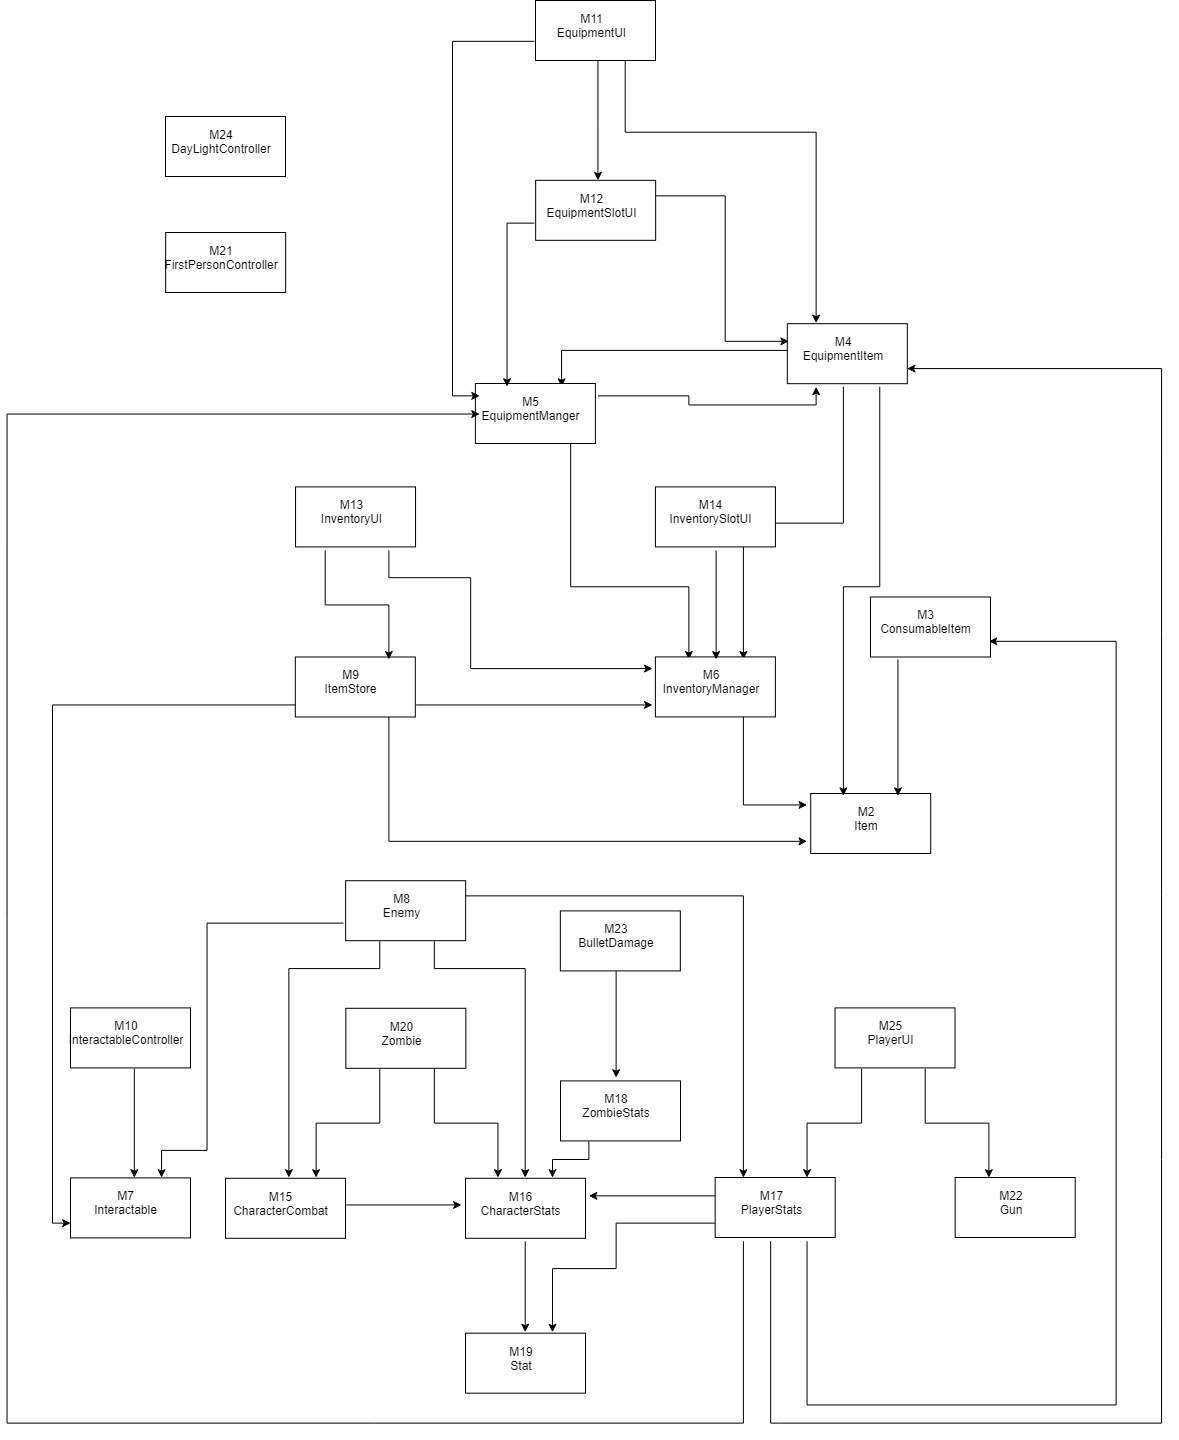
\includegraphics[scale=0.3]{UsesHierarchy.png}
\caption{Use hierarchy among modules}
\label{FigUH}
\end{figure}

\begin{table}[H]
\centering
\begin{tabular}{p{0.2\textwidth} p{0.6\textwidth}}
\toprule
\textbf{Modules} & \textbf{Uses}\\
\midrule
\sout{\mref{mHH}} & ~\\
\mref{mSDI} & \sout{\mref{mSDIM}}\\
\mref{mSDCI} & \mref{mSDI}, \mref{mSDIM}\\
\mref{mSDEI} & \mref{mSDI}, \mref{mSDEM}, \sout{\mref{mBHESU}} {\color{magenta} \mref{mSDIM}}\\
\mref{mSDEM} & \mref{mSDIM}, \mref{mSDEI}\\
\mref{mSDIM} & \mref{mSDI}\\
\mref{mBHI} & ~\\
\mref{mBHE} & \mref{mBHCC}, \mref{mSDCS}, \mref{mSDPS}, \mref{mBHI}\\
\mref{mBHIS} & \mref{mSDI}, \mref{mBHI}, \mref{mSDIM}\\
\mref{mBHIC} & \mref{mBHI}\\
\mref{mBHEU} & \mref{mSDEM}, \mref{mBHESU}, {\color{magenta} \mref{mSDEI}}\\
\mref{mBHESU} & \mref{mSDEI}, \mref{mSDEM}\\
\mref{mBHIU} & \mref{mSDIM}, \mref{mBHIS}\\
\mref{mBHISU} & \mref{mSDIM}\\
\mref{mBHCC} & \mref{mSDCS}\\
\mref{mSDCS} & \mref{mSDS}\\
\mref{mSDPS} & \mref{mSDCS}, \mref{mSDS}, \mref{mSDEM}, \mref{mSDCI}, \mref{mSDEI}\\
\mref{mSDZS} & \mref{mSDCS}\\
\mref{mSDS} & ~\\
\mref{mBHZ} & \mref{mBHCC}, \mref{mSDCS}\\
\mref{mBHFPS} & ~\\
\mref{mBHG} & ~\\
\mref{mBHBD} & \mref{mSDZS}\\
{\color{magenta} \mref{mBHDLC}} & ~\\
{\color{magenta} \mref{mBHPU} }& {\color{magenta} \mref{mSDPS}, \mref{mBHG}}\\
\bottomrule
\end{tabular}
\caption{Use hierarchy among modules in table format for Figure \ref{FigUH}}
\label{TblACT}
\end{table}

{\color{magenta} \mref{mSDEI} and \mref{mSDEM} use each other. \\
\mref{mSDEI} has a method that defines that when an equipment item is used, it is equipped. The method for equipping an item is in \mref{mSDEM}. \\
\mref{mSDEM} uses \mref{mSDEI} because since \mref{mSDEM} deals with equipping and unequipping equipment items, \mref{mSDEM} needs to use the class type defined in \mref{mSDEI} to do so.}

%\section*{References}

\bibliographystyle {plainnat}
\bibliography {MG}

\end{document}
